\documentclass[../main.tex]{subfiles}

\tikzset
  {phase/.style={draw,minimum width=2.5cm,minimum height=1.5cm,align=center}
  ,previous/.style={below right=0.5cm of #1}
  }
\newcommand\connecttw[2]%
  {\draw[->,thick] (#1) -| (#2);
   \draw[->,thick] (#2) -| (#1);
  }
\newcommand\connectow[2]%
  {\draw[thick, ->] (#1) |- (#2);
  }

\begin{document}
The following chapter introduces the Agile philosophy, including a comparison with traditional waterfall methods. The chapter then continues with the definition of Scrum methodology, giving a overview of the tools, processes and roles related to it.\\
The focus is going to be mainly software related, as those method originated as a way to efficiently develop software projects.
\section{The Agile philosophy}
By reading the previous lines we need to put extra effort into analyzing each word. 
\textit{Agile} has been coupled from the beginning of the Chapter only with \textit{philosophy}.  
The word philosophy emphasises the fact that we are referring to a way of thinking but also on the other hand that we are not trying to give any method to support this way of thinking. Then we have the word Agile, which firmly add dynamism to this way of thinking.\\ 
The Agile philosophy definition can be therefore reported as dynamic way based on iterative cycles to approach project development.
\subsection{History of the Agile methodology}
The definition of a word Agile as a theorized philosophy for product development came only in the early 90´as a result of the Agile Manifesto. It´s important to keep in mind that there where previously approaches that resemble, if not match Agile, those can be inserted under the umbrella term IID, \textit{Iterative Incremental Approaches}.\\
As most of the innovation also the IID ones come from the criticism of previously used methods. In the past most of the methodology to develop product and in particular to develop software where based on a series of sequential steps which output could only be seen at the end of the process. The series of steps was sometimes so long that the product was already out of the market once completed.\\
The criticism in regard to those methods suggested alternatives approaches which where actually unconsciously filled by Agile ideas such as the response to changes, customer involvement, and working software over documentation.\\
By reading the paper by \citet{larman2003iterative} the traces of iterative and incremental development approaches can already be found in the 30´. \\
Bell Labs, one of the center that provided the greatest innovation in recent history, the invention of the transistor is also the one who first applied with sufficient success IID method. Walter Shewahrt in 1930 posed a series of short "plan-do-study-act" (PSDA) cycles for quality improvement. This method was a great success and the PSDA was vigorously promoted starting from the 40.\\ 
Tanks to the success the next step for IID was to flood military projects. Iterative approaches were used in the development of the X-15 hyper-sonic jet in which the "Agile like" practices contributed majorly to its success.\\ Post war IDD experience and experts arrived at NASA, which in the 60´was US government top priority with the ongoing cold war.\\
Project Mercury, the first human spaceflight program of the United States, used short half day iterations. The Development Team performed technical review of all the changes, and applied a super early version of Extreme Programming practice of "test first" development. This consist in writing test before each micro increment. They also applied top-down development with the usage of stubs. Stubs simulate the behaviour of code or is used as a substitute to yet-to-be-developed code.\\ 
\section{Agile Manifesto}
The influences continued until a real theorizing was made in 2001 by software developer that, tired of inefficient way to develop software summed all up under the slogan "\textit{We are uncovering better ways of developing software by doing it and helping others do it}". \\
The proponents of the Manifest found them self in a situation in which no software development methodology or techniques enabled them to succeed in a constant manner. As reported \citet{schmidt2013software} the Manifesto was to established a guild surrounding a set of principles for software development based on rapid prototyping, incremental product delivery, and absolutely no product design. The Manifesto highlighted 4 values:
\begin{itemize}
    \item \textit{individuals and interactions over processes and tools.}
    \item \textit{working software over comprehensive documentation.}
    \item \textit{customer collaboration over contract negotiation.}
    \item \textit{responding to change over following a plan.}
\end{itemize}

\paragraph{Individuals and interactions over processes and tools}
One of Agile goals is the one to enhance the communications inside teams. With this principle this goal is underlined. The importance of having good interactions between the team members surpass the focus of having high-tech tools or complex processes. \\
The main problem with tools and process is that they push towards a certain conformity. 
Conformity makes it hard to accommodate new ideas, requirements and way of thinking. 
Other than that the more robust a process or a tool is, the more time it require to "translate" everything in order to fit it. 
Agile stays human-centric and team focused. Every member need to be an active participants. 
\paragraph{Working software over comprehensive documentation}
One of the flaws of waterfall method is that can happen that a working software version arrives when the initial requirements are already outdated. To criticize this mechanism it´s important to deeply working software as soon as possible during the development process. Having a working product as early as possible is also use full for getting customer feedback on it, as the next values will underline. 
It´s important to state that documentation don´t need to be completely left out but it´s important to focus more on what´s important and what´s not in terms of documentation artifacts. Documentation requires indeed not only a lot of time to be set up, but also to be maintained. 
\paragraph{Customer collaboration over contract negotiation}
This value stresses the importance of encouraging customer and developer team collaboration over the product, other than seeing each other as adversaries in the contract negotiation part.
Creating a strong customer relationship translates to more frequent and accurate customer feedback. The more a customer is involved in the product the more the outcome of a product is shared between developers and the customer itself. Thus the push in the direction of success is stronger.  
\paragraph{Responding to change over following a plan}
This stands as the most innovative values out of the four. The ability not only to respond to changes but to welcome it during the developing process is a really important tool for Agile. Differently from other approaches, as for example QFD, in Agile as time and knowledge over the product increases the ability to make changes stay unvaried. This is a really innovative concept. The cost related to changes ideally stay the same until product delivery. In traditional method this cost tend to infinite when getting near the product delivery.

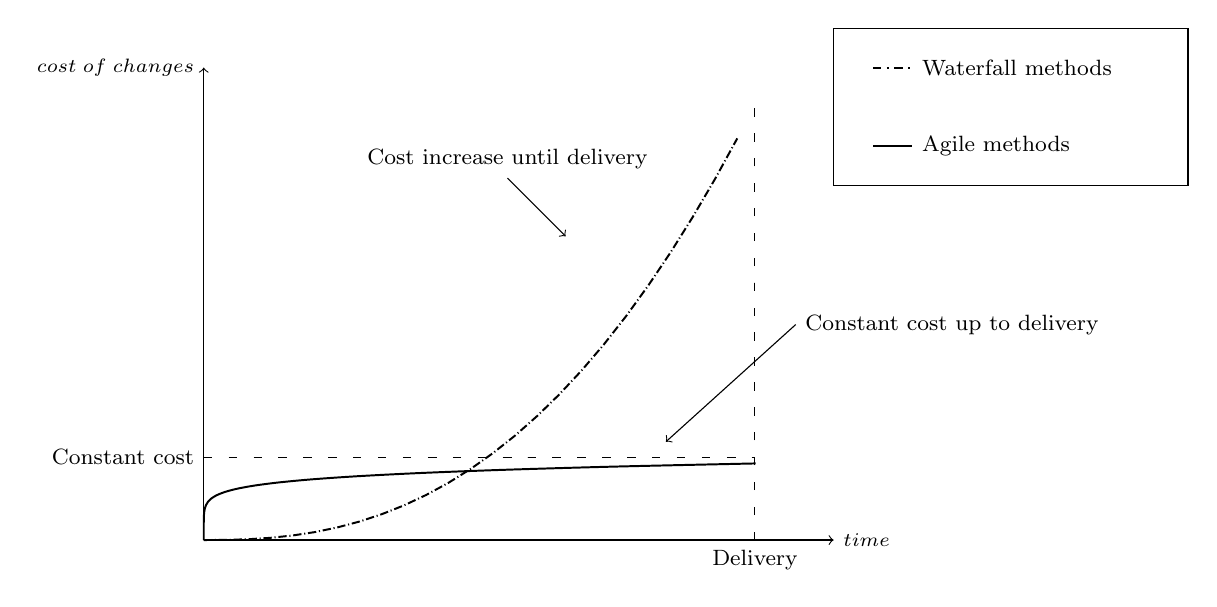
\begin{tikzpicture}
  \draw[->] (0, 0) -- (8, 0) node[right] {\scriptsize $time$};
  \draw[->] (0, 0) -- (0, 6) node[left] {\scriptsize $cost\;of\;changes$};
  \draw[scale=0.7, domain=0:2.42, densely dashdotted, line width=0.25mm, variable=\x, black] plot ({4*\x}, {0.8*\x^2.5});
  \draw[scale=0.7, line width=0.25mm, domain=0:1.39, smooth, variable=\y, black]  plot ({\y^7}, {\y});
  \draw[loosely dashed, scale=0.7, domain=0:10, smooth, variable=\y, black]  plot ({\y}, {1.5});
  \draw[loosely dashed, scale=0.7, domain=0:8, smooth, variable=\x, black]  plot ({10}, {\x});
  \node at (7,0) [align=center,anchor=north ] {\footnotesize Delivery};
  \node at (0,1.05) [align=center,anchor=east ] {\footnotesize Constant cost};
  \draw[<-] (40:6) -- (50:6) node[above] {\footnotesize Cost increase until delivery};
  \draw[<-] (12:6) -- (20:8) node[right] {\footnotesize Constant cost up to delivery};
  
  \draw [line width=0.25mm, dash dot] (8.5,6) -- (9,6);
  \node at (9,6) [right] {\footnotesize Waterfall methods};
  \draw [line width=0.25mm] (8.5,5) -- (9,5);
  \node at (9,5) [right] {\footnotesize Agile methods};
  \draw[draw=black] (12.5,6.5) rectangle ++(-4.5,-2);
 

  
\end{tikzpicture}


\subsection{Agile vs Waterfall methodology}


% \resizebox{\textwidth}{7cm}{
\begin{figure}
\centering
    \begin{tikzpicture}[>=stealth]
      \node[phase]                       (requirements) {\small Requirements};
      \node[phase,previous=requirements] (design)       {\small Design};
      \node[phase,previous=design]       (coding)       {\small Coding and\\unit test};
      \node[phase,previous=coding]       (integration)  {\small System\\integration};
      \node[phase,previous=integration]  (operation)    {\small Operation and\\maintenance};
      \connecttw{requirements}{design};
      \connecttw{design}{coding};
      \connecttw{coding}{integration};
      \connecttw{integration}{operation};
    \end{tikzpicture}
\caption{Agile model}
\end{figure}

\begin{figure}
\centering
    \begin{tikzpicture}[>=stealth]
     \node[phase]                       (requirements)  {\small Requirements};
      \node[phase,previous=requirements] (design)       {\small Design};
      \node[phase,previous=design]       (coding)       {\small Coding and\\unit test};
      \node[phase,previous=coding]       (integration)  {\small System\\integration};
      \node[phase,previous=integration]  (operation)    {\small Operation and\\maintenance};
      \connectow{requirements}{design};
      \connectow{design}{coding};
      \connectow{coding}{integration};
      \connectow{integration}{operation};
    \end{tikzpicture}
\caption{Waterfall model}
\end{figure}
% }
\section{Scrum}
As previously underlined, the Agile philosophy does not present a specific set of practices with which approach product (or software) development. Scrum, on the other hand, provides a structured framework to approach product development based on Agile principles.\\
The word frameworks intend to underline a concrete set of procedures that allow Agile like practises to be applied in a development process.\\
The definitions from the creators of Scrum (\citet{Scrum}) is the following:
\begin{quote}
\textit{Scrum is not a process, technique, or definitive method. Rather, it is a framework within which you can employ various processes and techniques. Scrum makes clear the relative efficacy of your product management and work techniques so that you can continuously improve the product, the team, and the working environment.}
\end{quote}
The Scrum framework consist of:
\begin{itemize}
    \item Scrum teams, a small group of people with a defined hierarchy. Each member has a particular role. 
    \item Events, the process of developing a product is scheduled thorough a series of meetings. The meeting sums up to compose a Scrum sprint.
    \item Rules, bind together the roles, events, and artifacts, governing the relationships and interaction between them.
\end{itemize}
\subsection{Scrum teams}
Scrum teams are composed by a Product Owner, the Development Team and a Scrum Master. Outside the Scrum team we find also A Business Owner, the Stakes-holder and the Subjects Matter Experts (SME). 
\begin{figure}[H]
    \centering
\tikzset{every picture/.style={line width=0.75pt}} %set default line width to 0.75pt        

\begin{tikzpicture}[x=0.75pt,y=0.75pt,yscale=-1,xscale=1]
%uncomment if require: \path (0,300); %set diagram left start at 0, and has height of 300

%Straight Lines [id:da20494949801039608] 
\draw    (365,106.2) -- (352.1,85.74) ;
\draw [shift={(350.5,83.2)}, rotate = 417.77] [fill={rgb, 255:red, 0; green, 0; blue, 0 }  ][line width=0.08]  [draw opacity=0] (8.93,-4.29) -- (0,0) -- (8.93,4.29) -- cycle    ;
%Shape: Circle [id:dp3857817213089323] 
\draw  [color={rgb, 255:red, 155; green, 155; blue, 155 }  ,draw opacity=1 ] (248.5,201.2) .. controls (248.5,152.88) and (287.68,113.7) .. (336,113.7) .. controls (384.32,113.7) and (423.5,152.88) .. (423.5,201.2) .. controls (423.5,249.52) and (384.32,288.7) .. (336,288.7) .. controls (287.68,288.7) and (248.5,249.52) .. (248.5,201.2) -- cycle ;
%Image [id:dp3791077254508246] 
\draw (312.75,221.1) node  {
\includegraphics[width=34.88pt,height=29.85pt]{2101886Untitled-3-512.png}};
%Image [id:dp3637136401430079] 
\draw (337.25,222.1) node  {
\includegraphics[width=34.88pt,height=29.85pt]{2101886Untitled-3-512.png}};
%Image [id:dp12188126083600448] 
\draw (359.25,221.1) node  {
\includegraphics[width=34.88pt,height=29.85pt]{2101886Untitled-3-512.png}};
%Image [id:dp23894019368631736] 
\draw (340.25,64.1) node  {
\includegraphics[width=34.88pt,height=29.85pt]{2101886Untitled-3-512.png}};
%Image [id:dp1300496672968483] 
\draw (397.75,65.1) node  {
\includegraphics[width=34.88pt,height=29.85pt]{2101886Untitled-3-512.png}};
%Image [id:dp9876721113766473] 
\draw (421.25,67.1) node  {
\includegraphics[width=34.88pt,height=29.85pt]{2101886Untitled-3-512.png}};
%Image [id:dp31174606939750626] 
\draw (443.25,65.1) node  {
\includegraphics[width=34.88pt,height=29.85pt]{2101886Untitled-3-512.png}};
%Image [id:dp37861138210159484] 
\draw (193.25,136.1) node  {
\includegraphics[width=34.88pt,height=29.85pt]{2101886Untitled-3-512.png}};
%Image [id:dp5522485177346022] 
\draw (193.25,188.1) node  {
\includegraphics[width=34.88pt,height=29.85pt]{2101886Untitled-3-512.png}};
%Image [id:dp27943172444988784] 
\draw (194.25,238.1) node  {
\includegraphics[width=34.88pt,height=29.85pt]{2101886Untitled-3-512.png}};
%Straight Lines [id:da6490226371262615] 
\draw  [dash pattern={on 4.5pt off 4.5pt}]  (311,105) -- (327.61,84.53) ;
\draw [shift={(329.5,82.2)}, rotate = 489.06] [fill={rgb, 255:red, 0; green, 0; blue, 0 }  ][line width=0.08]  [draw opacity=0] (8.93,-4.29) -- (0,0) -- (8.93,4.29) -- cycle    ;
%Image [id:dp810647601013762] 
\draw (304.25,123.1) node  {
\includegraphics[width=34.88pt,height=29.85pt]{2101886Untitled-3-512.png}};
%Image [id:dp7726630656533122] 
\draw (374.25,123.1) node  {
\includegraphics[width=34.88pt,height=29.85pt]{2101886Untitled-3-512.png}};
%Straight Lines [id:da8895253755438801] 
\draw    (213.68,141.26) -- (245.32,171.14) ;
\draw [shift={(247.5,173.2)}, rotate = 223.36] [fill={rgb, 255:red, 0; green, 0; blue, 0 }  ][line width=0.08]  [draw opacity=0] (8.93,-4.29) -- (0,0) -- (8.93,4.29) -- cycle    ;
\draw [shift={(211.5,139.2)}, rotate = 43.36] [fill={rgb, 255:red, 0; green, 0; blue, 0 }  ][line width=0.08]  [draw opacity=0] (8.93,-4.29) -- (0,0) -- (8.93,4.29) -- cycle    ;
%Straight Lines [id:da566128210538136] 
\draw    (214.5,191.2) -- (241.5,191.2) ;
\draw [shift={(244.5,191.2)}, rotate = 180] [fill={rgb, 255:red, 0; green, 0; blue, 0 }  ][line width=0.08]  [draw opacity=0] (8.93,-4.29) -- (0,0) -- (8.93,4.29) -- cycle    ;
\draw [shift={(211.5,191.2)}, rotate = 0] [fill={rgb, 255:red, 0; green, 0; blue, 0 }  ][line width=0.08]  [draw opacity=0] (8.93,-4.29) -- (0,0) -- (8.93,4.29) -- cycle    ;
%Straight Lines [id:da8445013462809028] 
\draw    (213.82,239.29) -- (243.18,215.11) ;
\draw [shift={(245.5,213.2)}, rotate = 500.53] [fill={rgb, 255:red, 0; green, 0; blue, 0 }  ][line width=0.08]  [draw opacity=0] (8.93,-4.29) -- (0,0) -- (8.93,4.29) -- cycle    ;
\draw [shift={(211.5,241.2)}, rotate = 320.53] [fill={rgb, 255:red, 0; green, 0; blue, 0 }  ][line width=0.08]  [draw opacity=0] (8.93,-4.29) -- (0,0) -- (8.93,4.29) -- cycle    ;
%Straight Lines [id:da7042199192540972] 
\draw    (360.5,66.32) -- (378.5,67.08) ;
\draw [shift={(381.5,67.2)}, rotate = 182.39] [fill={rgb, 255:red, 0; green, 0; blue, 0 }  ][line width=0.08]  [draw opacity=0] (8.93,-4.29) -- (0,0) -- (8.93,4.29) -- cycle    ;
\draw [shift={(357.5,66.2)}, rotate = 2.39] [fill={rgb, 255:red, 0; green, 0; blue, 0 }  ][line width=0.08]  [draw opacity=0] (8.93,-4.29) -- (0,0) -- (8.93,4.29) -- cycle    ;

% Text Node
\draw (283,240) node [anchor=north west][inner sep=0.75pt]   [align=left] {Developer team};
% Text Node
\draw (278,139) node [anchor=north west][inner sep=0.75pt]   [align=left] {Scrum\\Master};
% Text Node
\draw (347,139) node [anchor=north west][inner sep=0.75pt]   [align=left] {Product\\Owner};
% Text Node
\draw (465,57) node [anchor=north west][inner sep=0.75pt]   [align=left] {Stakeholders};
% Text Node
\draw (206,57) node [anchor=north west][inner sep=0.75pt]   [align=left] {Business Owner};
% Text Node
\draw (173,261) node [anchor=north west][inner sep=0.75pt]   [align=left] {SME};


\end{tikzpicture}
    \caption{Scrum team structure}
\end{figure}
Scrum Teams are a self-organizing and cross functional. The self organization is needed to better decide with the team how to get work done, rather than having this decided from the outside.\\
Cross-functional team have all competencies needed to complete the task. A team need to be composed by what \citeauthor{Scrumastery} defines as T-shaped people. The name comes from the fact that the vertical shaft of the T represent the depth of their chosen preferred skill, while the horizontal bar of the T represents the diversity of other skills they can dip into in order to collaborate. Obviously T-shaped people antagonist are the I-shaped people, that have a set of skills, therefore, that is deeper than broad, resembling the letter I.\\
The sole goal of Scrum teams is to deliver products iteratively and incrementally, maximizing opportunities for feedback. 
\begin{figure}
\centering
\begin{minipage}{.5\textwidth}
  \centering
 \tikzset{every picture/.style={line width=0.75pt}} %set default line width to 0.75pt        

\begin{tikzpicture}[x=0.75pt,y=0.75pt,yscale=-0.7,xscale=0.7]
%Shape: Rectangle [id:dp793644495324062] 
\draw   (318,25.2) -- (387,25.2) -- (387,215.2) -- (318,215.2) -- cycle ;
% Text Node
\draw (191,35) node [anchor=north west][inner sep=0.75pt, yscale=0.7,xscale=0.7]   [align=left] {Design \ \ Analysis \ \ Develop \ \ Test \ \ Architect};
\end{tikzpicture}
  \caption{I-shaped person}
\end{minipage}%
\begin{minipage}{.5\textwidth}
  \centering
\tikzset{every picture/.style={line width=0.75pt}} %set default line width to 0.75pt        
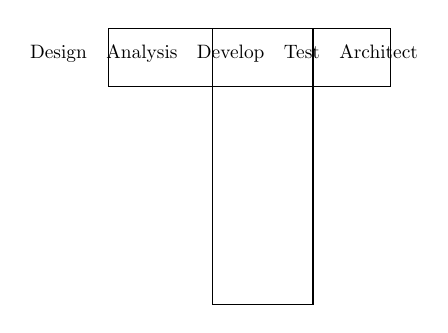
\begin{tikzpicture}[x=0.75pt,y=0.75pt, yscale=-0.7,xscale=0.7]
%Shape: Rectangle [id:dp793644495324062] 
\draw   (318,25.2) -- (387,25.2) -- (387,215.2) -- (318,215.2) -- cycle ;
%Shape: Rectangle [id:dp3939879341512962] 
\draw   (246.5,25) -- (440.5,25) -- (440.5,65.2) -- (246.5,65.2) -- cycle ;
% Text Node
\draw (191,35) node [anchor=north west][inner sep=0.75pt, yscale=0.7,xscale=0.7]   [align=left] {Design \ \ Analysis \ \ Develop \ \ Test \ \ Architect};
\end{tikzpicture}
  \caption{T-shaped person}
\end{minipage}
\end{figure}

\subsection{The product owner}
The Product Owner is responsible for maximizing the value of the product resulting from work of the Development Teams. This encompasses managing the Product Backlog (the concept will be later explained). The product owner decisions can be seen from the Backlog organization, giving a clear overview to the team and to the business owner of the work.\\
\subsection{The Development Team}
The Development Team consist of professionals who do the work of delivering a potentially releasable Increment of "Done" product at the end of each sprint. Only the members of the Development Team can deliver a product increment. \\
The Development Team need the following characteristics:
\begin{itemize}
    \item They are self-organizing. A potentially releasable functionality is chosen from the members, not even the Scrum Master can influence this choice. 
    \item Development Teams need to be cross-functional. 
    \item Accountability belongs to the Development Team as a whole. 
\end{itemize}
Scrum teams size is small enough to remain nimble and large enough to complete work in the Sprint.
\subsection{The Scrum Master}
Scrum Master is responsible for promoting and supporting Scrum. Scrum Masters do this by helping everyone understand Scrum theory, practices, rules and values. 
The Scrum Master role is to interface between the Scrum Team and those on the outside, his success is related to the success in the interactions, in order to maximize the value created by the Scum Team. The following interfaces roles are required to the Scrum Master:
\begin{itemize}
    \item Scrum Master to the Product Owner, ensuring that goals, scope and product domain are understood by the Product Owner and the Backlog resealable those objectives.
    \item Scrum Master to the Development Team, coaching team on self-organization and cross-functionality while outputting high quality products. 
    \item Scrum Master to the Organization, helping stakeholder understand the empirical product development and work and act as an intermediary for the communication from outside to the Scrum team. 
\end{itemize}

\subsection{Scrum Process}
\subsection{Scrum tools}
\subsection{Scrum roles}
\section{Direct application of Agile for software development}
\cleardoublepage
\end{document}